
\documentclass[a4paper, 9pt]{extarticle}

\usepackage{extsizes}
\usepackage[a4paper, total={6.5in, 10in}]{geometry}

\usepackage{graphicx}
\usepackage{listings}
\usepackage{xcolor}
\usepackage{ textcomp } % For text 1/2
\newcommand{\code}{\texttt}
\newcommand{\str}[1]{\texttt{'#1'}}

%New colors defined below
\definecolor{codegreen}{rgb}{0,0.6,0}
\definecolor{codegray}{rgb}{0.5,0.5,0.5}
%\definecolor{codepurple}{rgb}{0.58,0,0.82}
\definecolor{codeorange}{rgb}{0.75, 0.51, 0.15}
\definecolor{codered}{rgb}{0.5, 0, 0}
\definecolor{backcolour}{rgb}{0.95,0.95,0.92}

\lstset{
  backgroundcolor=\color{backcolour},
  commentstyle=\color{codegreen},
  keywordstyle=\color{codeorange},
  numberstyle=\tiny\color{codegray},
  stringstyle=\color{codered},
  basicstyle=\ttfamily\scriptsize,
  breakatwhitespace=false,         
  breaklines=true,                 
  captionpos=b,                    
  keepspaces=true,                 
  numbers=left,                    
  numbersep=5pt,                  
  showspaces=false,                
  showstringspaces=false,
  showtabs=false,                  
  tabsize=2,
  inputencoding=utf8,
  extendedchars=false,
  escapeinside={\%*}{*)},
}

\title{
Data Mining Project\\
Text Normalization Challenge\\
\large Converting text from written expressions into spoken forms}

\author{Tom Aarsen - s1027041}
\date{December 2019}

\begin{document}

\maketitle
\section{Abstract}\vspace{-1mm}
This paper proposes a method for solving, as well as a solution to, a text-to-speech normalization problem, which focuses on converting text from written expressions into spoken forms. The method parses input tokens through a gradient boosted decision tree model, which classifies the token as one of 16 different types of tokens. The token is then converted based on the predicted token type, resulting in a normalized output of the spoken form. Upon entering a related text-to-speech normalization competition, the solution achieved an accuracy of \code{99.590\%}, placing 12th out of the 260 teams, or within the top 5\% of all submissions.

\section{Research problem}\vspace{-1mm}
Natural language processing (NLP) is a well-known tough subfield of artificial intelligence and computer science, made especially difficult by human's preference for abbreviations and contractions. One of the many challenging problems within NLP is converting written text containing such abbreviations and contractions to a spoken representation, using a process called text normalization. Such a representation is required for text-to-speech (TTS) and automatic speech recognition (ARS) systems to be able to convert spoken words into written text, and vice versa.\\
\\
These systems have broad use cases, ranging from aiding the visually impaired to digital assistants, with many large parties interested in advancing the field of text normalization. One such party is Google, whose Text Normalization Research Group sponsored an English Language Text Normalization Challenge\footnote{The competition: https://www.kaggle.com/c/text-normalization-challenge-english-language} on the machine learning competition website Kaggle. Alongside a monetary prize, they donated several datasets totalling some 12 million entries.

\subsection{Previous research}\vspace{-1mm}
The sponsors themselves have published research on this problem in the previous years:
\begin{itemize}
    \itemsep-0.3em
    \item Wu, Gorman, and Sproat (2016)\footnote{Wu, Gorman, and Sproat (2016): https://arxiv.org/abs/1609.06649} proposes a model with hand-written grammars with all possible verbalizations per token, with a corpus of written-spoken utterances, used to train a ranking model that selects the most appropriate verbalization given the context.
    \item Gorman and Sproat (2016)\footnote{Gorman and Sproat (2016): https://www.transacl.org/ojs/index.php/tacl/article/view/897/213} proposes two models for verbalizing numbers, one with a recurrent neural network and one with finite-state transducers. The main difference found between the two options is the amount of data required to train the models effectively.
    \item Sproat and Jaitly (2017)\footnote{Sproat and Jaitly (2017): https://arxiv.org/abs/1611.00068} proposes two recurrent neural network architectures trained on data sets very similar to the one used in this competition. Contraining the model with some grammar gives the best results.
\end{itemize}
\subsection{Data}
The competition contained 3 datasets: one training set and two testing sets.\\
The training set consists of 5 features:\\
\begin{tabular}{ll}
$\bullet$ \code{sentence\_id} & The index of the sentence this token belongs to. \\
$\bullet$ \code{token\_id} & The index of the position within this sentence this token belongs to.\\
$\bullet$ \code{before} & The original, raw text.\\
$\bullet$ \code{after} & The normalized text.\\
$\bullet$ \code{class} & The class to which this token belongs. \\
\end{tabular}\\
The testing sets only have the first 3 features. The goal of the competition is to predict the \code{after} column from the test sets. Note that the test set does not contain the \code{class} feature to help with predicting \code{after}.
\begin{minipage}[t]{0.5\textwidth}
\begin{lstlisting}[linewidth=26em]
sentence_id token_id     class     before               after
          5        0      DATE       2008  two thousand eight
          5        1     PLAIN       Tour                Tour
          5        2     PLAIN       with                with
          5        3     PLAIN     Madina              Madina
          5        4     PLAIN       Lake                Lake
          5        5     PUNCT          ,                   ,
          5        6     PLAIN     Coheed              Coheed
          5        7     PLAIN        and                 and
          5        8     PLAIN    Cambria             Cambria
          5        9     PLAIN        and                 and
          5       10     PLAIN  Fightstar           Fightstar
          5       11     PUNCT          .                   .
          6        0     PLAIN      Greek               Greek
          6        1     PLAIN   National            National
          6        2     PLAIN       Road                Road
          6        3  CARDINAL         91          ninety one
          6        4     PUNCT          (                   (
          6        5     PLAIN     Athens              Athens
          6        6     PUNCT          -                   -
          6        7     PLAIN     Sounio              Sounio
        ...      ...       ...        ...                 ...
\end{lstlisting}
%The following is a sample from the training set
\textit{A sample from the training set.}
\end{minipage}
\quad\quad\quad\quad\quad\quad\quad\quad\quad\
\begin{minipage}[t]{0.5\textwidth}
%while the following is a sample from one of the test sets:\\
\begin{lstlisting}[linewidth=15em]
sentence_id  token_id        before
         20         0            On
         20         1  May 20, 2008
         20         2             ,
         20         3           the
         20         4           DOI
         20         5     announced
         20         6          that
         20         7            it
         20         8         would
         20         9          take
         20        10        13,004
         20        11         acres
         20        12             (
         20        13     52.63 km2
         20        14             )
         20        15          into
         20        16         trust
         20        17             .
        ...       ...           ...
\end{lstlisting}
\textit{A sample from the testing set.}
\end{minipage}\\
\\
The correct predictions for \code{after} on the testing sets are not public, and hence these testing sets cannot be used for validation during development. They are only used to generate a submission for the competition.\\\\
Note that the \code{before} is usually just one word, but also often a sequence of words. From now on, the entire input section will be referred to as a token.

\subsection{Classes}
\label{DataClasses}
As can be seen in the training set sample, several classes exist. In total, there are 16:\\

\begin{minipage}{0.35\textwidth}
% Left
\small
\begin{tabular}{l|r}
\textbf{class}&\textbf{count}\\ \hline  
PLAIN       & 7353693\\ \hline  
PUNCT       & 1880507\\ \hline  
DATE        &  258348\\ \hline  
LETTERS     &  152795\\\hline
CARDINAL    &  133744\\\hline
VERBATIM    &   78108\\\hline
MEASURE     &   14783\\\hline
ORDINAL     &   12703\\\hline
DECIMAL     &    9821\\\hline
MONEY       &    6128\\\hline
DIGIT       &    5442\\\hline
ELECTRONIC  &    5162\\\hline
TELEPHONE   &    4024\\\hline
TIME        &    1465\\\hline
FRACTION    &    1196\\\hline
ADDRESS     &     522\\
\end{tabular}
\end{minipage}%
\begin{minipage}{0.55\textwidth}
% Right
The classes define the kind of normalization that should be applied on the token for a correct result. For instance, not every \str{20} should be converted in the same way. If the token is of the \code{CARDINAL} class, the correct result is \str{twenty}. However, if the class is \code{ORDINAL}, the output should be \str{twentieth}, and if the class is \code{DIGIT}, the correct output is \str{two o}.\\\\
Furthermore, in some cases there are even different results for the same input, within the same class. For instance, the raw text \str{\#} belonging to the \code{VERBATIM} class sometimes convert to \str{number}, and sometimes to \str{hash}.\\\\
It's clear that context matters.
\end{minipage}%

\section{Approach}
Rather than converting tokens straight from raw text to normalized text, raw tokens will be used to determine to which class the token belongs to. This predicted class will then determine the type of normalization applied on the token. This allows us to partition the tokens, and split up one massive conversion algorithm into 16 smaller ones, each serving a specific purpose, to convert text of that class to the correct output.\\
\\
Essentially the problem is split up from converting raw text to normalized text into two sub-problems: a classification problem to find the class, and a conversion problem to convert text from some class to the normalized text. In doing so, the range of the learning part of the problem can be reduced from several million to 16, which will heavily reduce overfitting before I even start, and make the job of the classifier significantly easier.

\subsection{Classification}
%Due to the flexibility afforded by neural networks, as the performance with non-linear relations is 
%A neural network's performance

Several aspects influenced by decisions regarding how I planned to tackle this classification problem.
\begin{enumerate}
    \itemsep-0.2em
    \item A lot of data is available to train on. 
    \item The relations between inputs and classes are non-trivial. 
    \item As mentioned in section \ref{DataClasses} Classes, the same input token can belong to different classes, depending on the context. Hence, the algorithm needs to be able to handle context. 
\end{enumerate}
A neural network would thrive given item 1, and such a network would not struggle with item 2 as much as other options like regression. To solve item 3, I veered towards a recurrent neural network (RNN). Such a network will get the result from previous words passing through the network as additional inputs. This allows it to use the classes of previous words to classify the current word.\\
\subsubsection{Recurrent Neural Networks}
A popular type of recurrent neural network is a long short-term memory (LSTM) network. Such a network is considerably better at preserving information from previous iterations as compared to more standard RNN networks. A LSTM cell contains a cell state acting as a conveyor belt of information, running through the entire cell and into the next cells. Information can easily pass along it unchanged. Beyond output data for words, also input data may be placed on this conveyor belt. This allows a neural network containing a layer of LSTM units to use this contextual information when deciding to which class the current token belongs.\\
\\
For this reason, the first attempt of a classification algorithm was a neural network containing such an LSTM layer. The implementation used Python's keras module, which takes some nested array of integers as input. This meant each token had to be split up into characters, each of which would be represented as the integer representation of said character. However, for the input to be valid, every array representation of a token must have the same length. This meant that every array had to be padded in some way to some predefined length. Another consequence was that every character after this point would be truncated.\\
Another problem with these LSTM layers is that the learned information would persist between sentences, even if the sentences are completely unrelated. For this reason I also tried to pad the space between sentences with empty words to allow the network to learn to forget at those points.\\
\\
Upon setting this predefined length to 32 characters, enough to not have to truncate 99.992\% of the training data, I started training with hold-out validation, using 90\% of the data as training data, while the remaining 10\% became validation or test data. After messing with each layer's hyperparameters, and trying different kinds of layers in addition to the LSTM layer, the best result I could get was an accuracy of 94\%. \\
\\
As this was not in line with the performance I was after, I quickly discarded the idea of using custom neural networks using keras and LSTM networks, and tried to find something else.

\subsubsection{Random Forests}
The next step was looking at random forests. I knew these had a good track record for machine learning competitions, even though one might think they are better at problems with more trivial, linear relations. However, the step from a LSTM network to a random forest meant that I lost the LSTM's natural ability to preserve information about previous tokens.\\
\\
I prepended each token with the previous token, and appended the two next tokens. This way there would be some contextual information present. However, with 4 tokens instead of just one, the length of each value to train on is very large. To combat this, each token was truncated. Using more characters means more information can be extracted from the data, but also increases memory use such that less data can be used to train on at a time. Using just the first 5 characters, with 4 tokens, proved to give the best results, when training using as much data as my GPU's memory can hold.\\
\\
I used a relatively popular module for random forests named XGBoost, which supports GPU learning and can plot feature importance. This latter allowed me to find out which features were useful.\\
\\
This method allowed me to get results nearing 99.4\% accuracy using 50\% of the data as training data, and the remaining 50\% as testing data. However, while browsing XGBoost's documentation during development, I found out about XGBoost's real bread and butter: training gradient-boosted decision trees. Although similar in representation, this method uses a different training algorithm.

\subsubsection{Gradient Boosted Decision Trees}
The interface between the two methods is very similar, so switching was not difficult. Using XGBoost's \code{XBGClassifier} I was able to achieve an accuracy of 99.78\%, using the same data features as with the random forest, and after some hyperparameter tuning.

\subsubsection{Classification Results}
The best model was trained using the 5750000 first tokens out of the total 9918441, of the training set, or roughly 57\%. The remaining 43\% was used as a testing set. This method proved to give better results than picking 57\% of each class, as well as taking all instances from the not as frequent classes, and then take some amount of PLAIN class tokens until 5.75 million tokens was reached.\\
As mentioned earlier, using the previous word as well as the two next words, where each word is represented as just the first 5 characters proved to give the best results both on the testing portion of the training dataset, and on the private testing set for the competition.\\
XGBoost allows for the plotting of features based on their relative gain within the model:\\
\includegraphics[scale=0.7]{FeatureImportanceV1Gain100dpi.png}\\
As can be seen, the meta-information about the word is considerably more useful than the characters of the previous and next words. Replacing the characters of the previous and next words with the meta-information of those tokens gives worse results both on the testing section of the training data as well as the private test set of the competition.\\
The following confusion matrix contains only values from the testing portion of the training data. For clarity, this data was not used to train on.\\
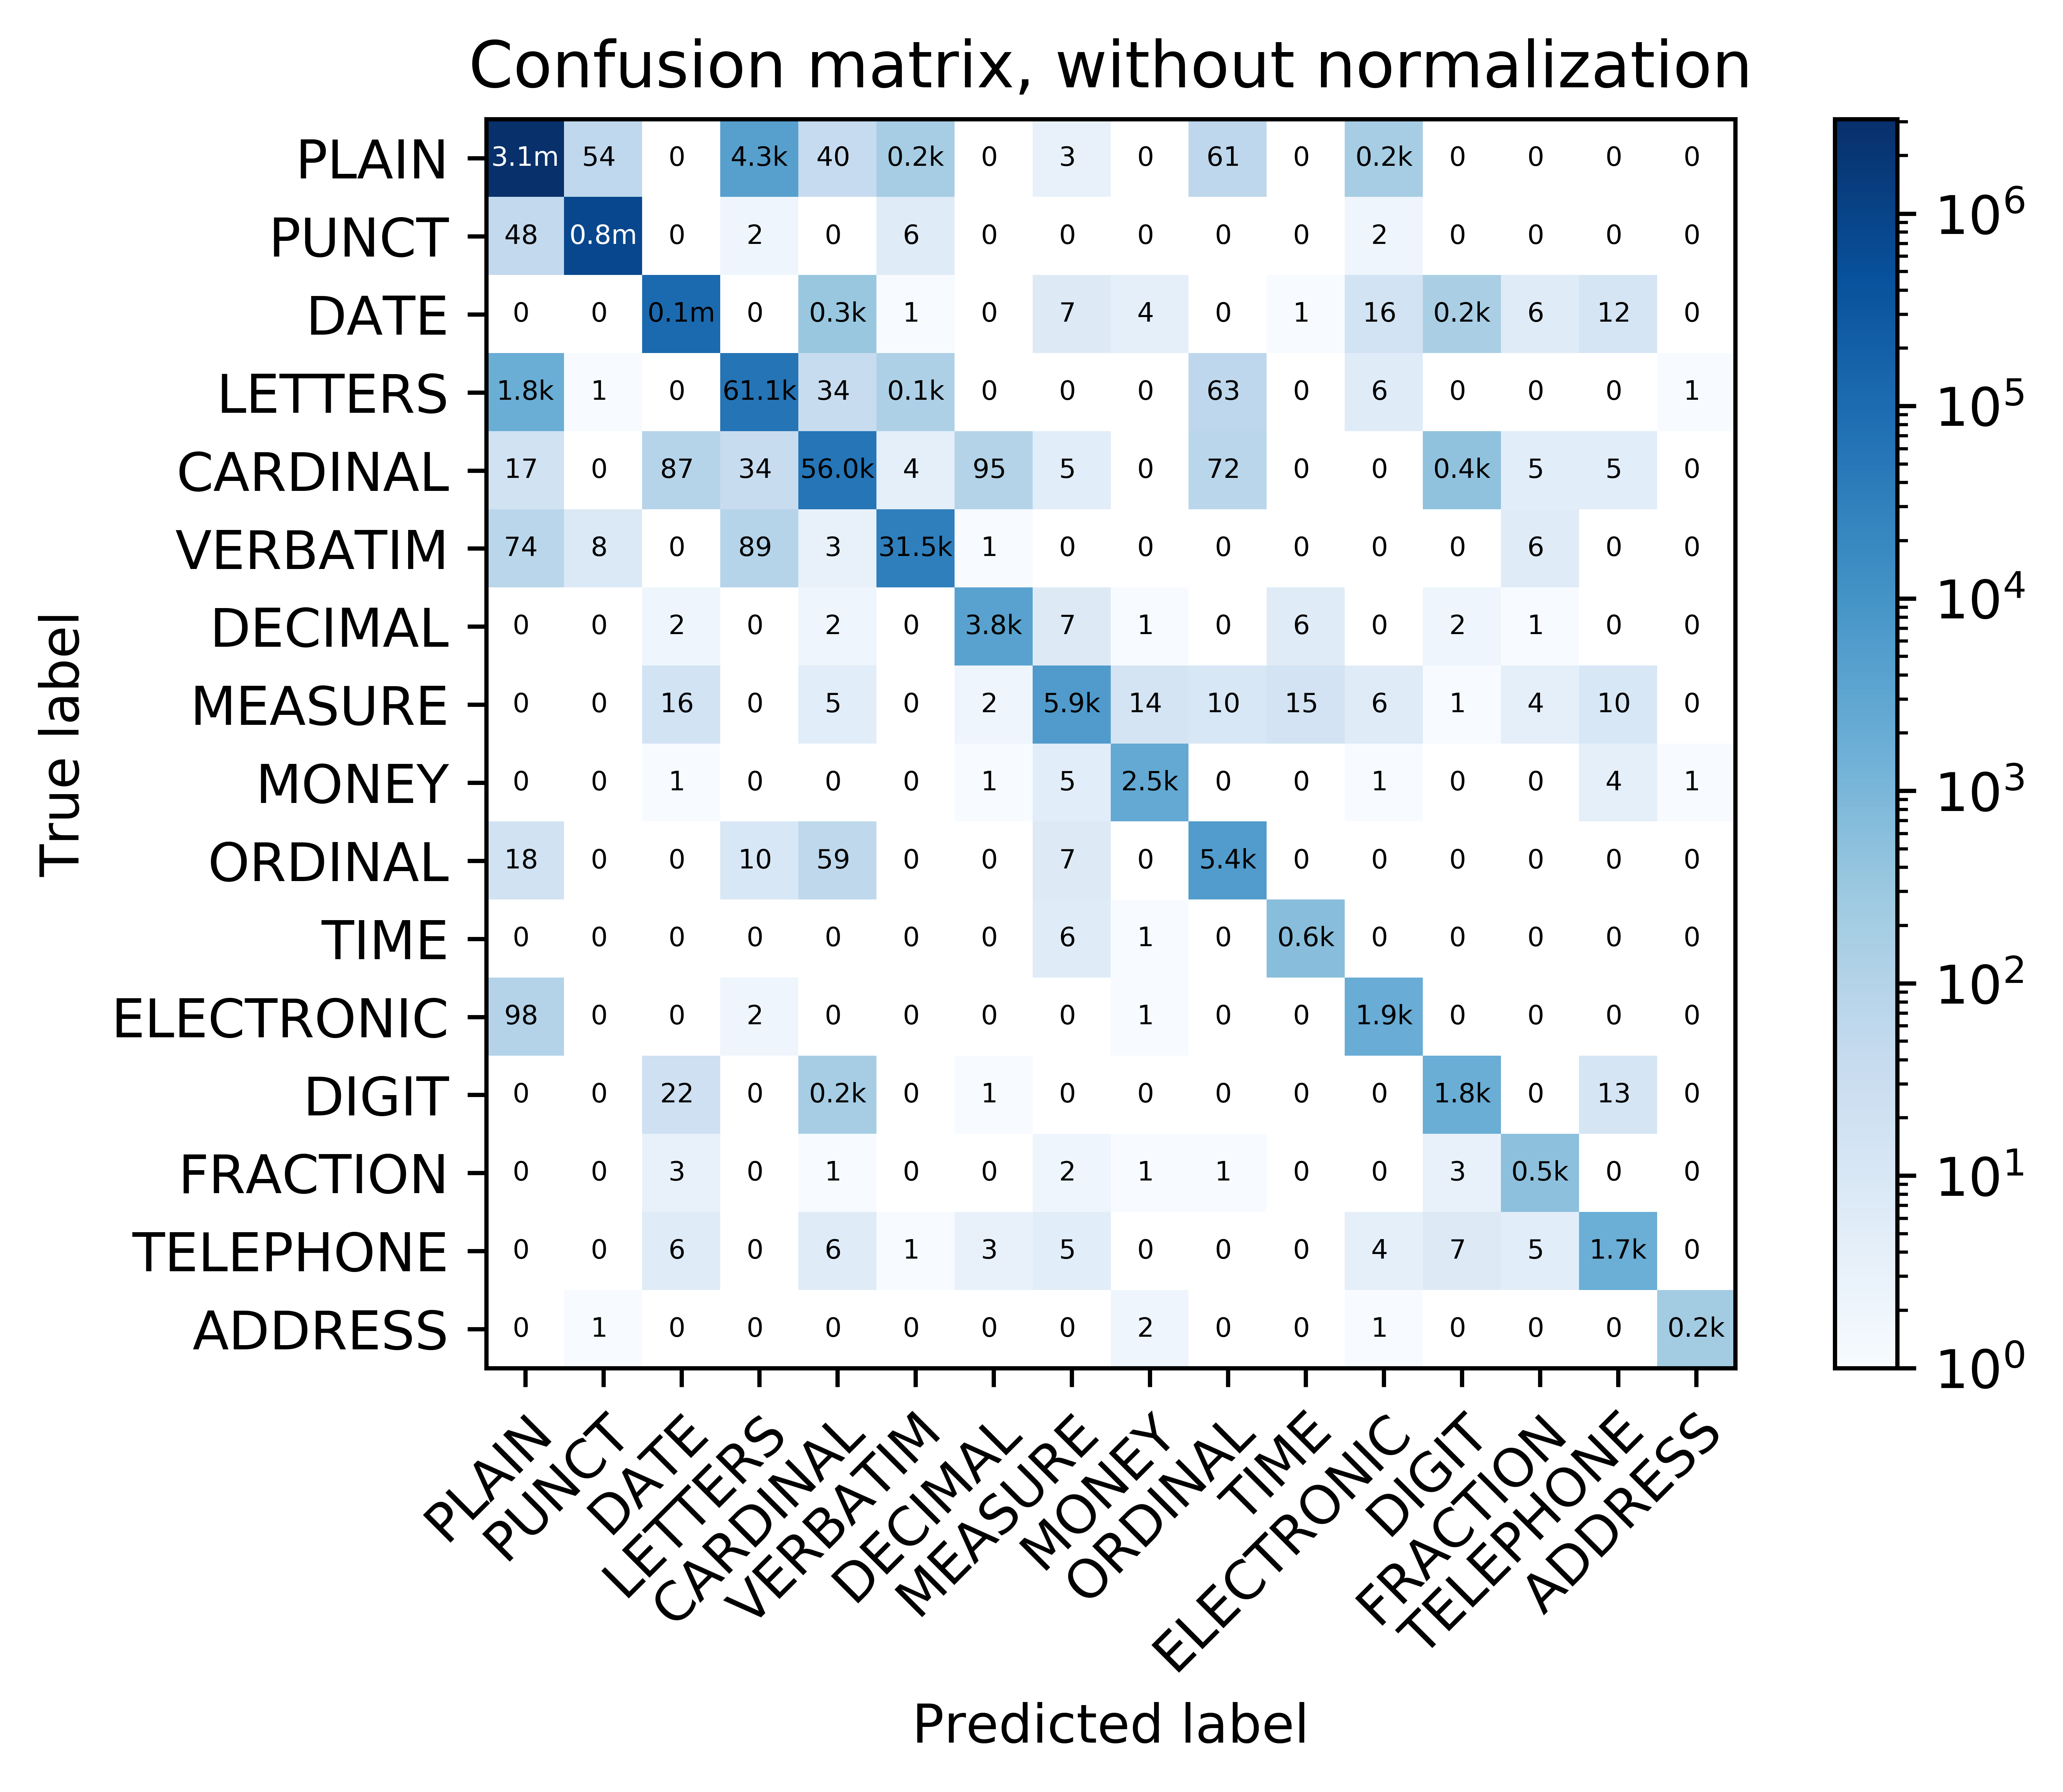
\includegraphics[scale=1]{ConfusionMatrix_v1_limit_bigfont.png}\\

\begin{minipage}{0.35\textwidth}
% Left
\begin{tabular}{l|l}
\textbf{class}&\textbf{AUC}\\ \hline  
PLAIN       & 0.998890\\ \hline  
PUNCT       & 0.999979\\ \hline  
DATE        & 0.999691\\ \hline  
LETTERS     & \textbf{0.984988}\\\hline
CARDINAL    & 0.997124\\\hline
VERBATIM    & 0.997904\\\hline
MEASURE     & 0.998406\\\hline
ORDINAL     & 0.991848\\\hline
DECIMAL     & 0.992617\\\hline
MONEY       & 0.998041\\\hline
DIGIT       & \textbf{0.942841}\\\hline
ELECTRONIC  & \textbf{0.978879}\\\hline
TELEPHONE   & 0.994407\\\hline
TIME        & 0.992491\\\hline
FRACTION    & \textbf{0.988712}\\\hline
ADDRESS     & 0.998084\\
\end{tabular}
\end{minipage}%
\begin{minipage}{0.615\textwidth}
% Right
The model gives binary outputs, so no useful ROC curve can be computed for them, as it would only have one point.\\
However, a table of AUC (Area Under Curve) values is still interesting. All values under 0.99 have been turned to bold. It shows that especially \code{DIGIT} is relatively often misclassified. The same can be seen in the Confusion matrix above, which shows that \code{CARDINAL} and \code{DIGIT} are often mixed up.\\
\\
\code{ELECTRONIC} is the second worst, as it sometimes predicts \code{PLAIN} instead, or vice versa. Adding an additional bit of meta-information stating whether the token matches a simple URL template might allow a model to get a slightly better performance here, at the cost of some additional memory used per token during learning.\\
\\
\code{FRACTION} is also below 0.99, but seems to only be due to outliers. The low amount of total instances of this class are the culprit of this relatively low AUC.\\
\end{minipage}\\\\
Lastly \code{LETTERS} are below 0.99, which are misclassified with \code{PLAIN} often. A total of 6133 times. Considering the sheer size of both of these classes, this is still a relatively small amount, but the misclassifications between \code{PLAIN} and \code{LETTER} account for 68.0764\% of all misclassifications.\\
This is to be expected, as the distinction between the \code{LETTER} and \code{PLAIN} class may even be difficult for humans.\\
\\
In the end, the total accuracy on the testing portion of the training dataset, which for clarification was not used in any training process, is 99.7838\%.

\subsection{Class-based token transformation}
Each token follows transformation rules specific to the class the token belongs to. The goal is now to make the best possible token transformation algorithm for each class, such that as many tokens belonging to each class are converted correctly. I will go over the steps taken to transform the tokens, give some examples and perhaps name some issues if applicable. Note that a more thorough explanation of the exact steps taken by the converters, as well as notes surrounding edge cases etc. is given in the source code in the Github\footnote{Github link: https://github.com/CubieDev/TTSTextNormalization}, for each converter. I would recommend having a look.\\
The proper conversion of tokens within each class is a difficult task to do with high accuracy, and has taken me a significant amount of time. 

\subsubsection{Plain class}
The plain class consists of all tokens that are simply words or abbreviations, that should be spoken as words. Because of this, 99.5030\% of all plain tokens are not modified between \code{before} and \code{after} at all.\\
The only transformations are converting words from the English spelling (eg "colour") to the American spelling (eg "color"), and converting abbreviations such as "wk" to "week".\\\\
The given data does seem to contain some oddities:
\begin{itemize}
    \itemsep-0.3em
    \item \str{Jan}, \str{Feb} and \str{Mar} are not converted to \str{january}, \str{february} and \str{march} respectively, while the other months of the year are converted to their full counterparts. I've opted to convert all months completely.
    \item Some names, such as \str{Elisabeth} and \str{Isaak} are normalized and converted to \str{elizabeth} and \str{izaak}. I've opted not to support this.
    \item Sometimes tokens like \str{NO} are converted to chemistry terms like \str{nitrogen monoxide}. I've opted not to support this.
\end{itemize}
Lastly, some tokens can only be correctly transformed within the proper context. For instance, \str{dr} may refers to \str{doctor} or to \str{drive}. Similarly with \str{st} referring to both \str{street} and \str{saint}. This context-based transformation is not supported in my algorithm, and the more common option is picked in these cases.\\
\\
All and all, 99.9882\% of all tokens are transformed correctly. If all cases where the \code{before} and \code{after} are identical are excluded, 97.8079\% of all tokens are correctly transformed.

\subsubsection{Punct class}
The punct class consists solely of punctuation, and is never modified between \code{before} and \code{after}. Hence, the accuracy here is 100\%.

\subsubsection{Date class}
The date class consists of dates in all kinds of formats. To name a few, the data includes \str{DD Month}, \str{MM-DD-YY(YY)}, \str{YY(YY)-MM-DD}, \str{DD-Month-YY(YY)}, \str{Month DD, YYYY}, \str{YYYYs}, \str{DD Month YYYY} and a ton more. Pretty much any kind of date format is included, and also supported by my converter.\\
Some unusual cases include \str{90s} or \str{2010s}, which need to be converted to \str{nineties} and \str{twenty tens} respectively, or \str{13 A.D.} which becomes \str{thirteen a d}. Additionally, some dates are prepended with the weekday or \str{the}.\\
\\
A total of 11 regular expressions can detect all of these cases, and parse the information. Once all days, months, years, prefixes, suffixes etc. have been extracted, one of two kinds of normalized translation can begin:
\begin{itemize}
    \itemsep-0.3em
    \item $\str{May 5 2010} \to \str{may fifth twenty ten}$
    \item $\str{5 May 2010} \to \str{the fifth of may twenty ten}$
\end{itemize}
In short, the order of the month and day within the input token affects the order of months and days in the output as well.\\
\\
In the end, the only incorrect cases are the following:
\begin{itemize}
    \itemsep-0.3em
    \item \str{7 A.D.} is parsed as \str{o seven a d} in the data. My converter returns \str{seven a d} instead. Essentially, whenever there is a suffix such as \str{AD}, and the year is a single character, in the data an \str{o} is prepended to the output.
    \item Sometimes dates such as \str{31/01/08} are converted to \str{the eighth of january thirty one} in the data. My converter returns \str{the thirty first of january o eight} instead, which I believe is the correct date.
    \item Sometimes an arbitrary suffix is included in the token, such as in \str{31 March 2014 A}. In this case, the data removes the A, while my converter keeps it.
\end{itemize}
The total accuracy of the date converter on all tokens of the date class within the training data is 99.9822\%.

\subsubsection{Letters class}
The letters class mostly consists of acronyms, and is generally converted by padding the alphabetical characters with spaces: \str{IUCN} $\to$ \str{i u c n}, as this is how a human would pronounce the input.\\
However, some cases are slightly different:
\begin{itemize}
    \itemsep-0.3em
    \item The character \str{é} is translated to \str{e acute}.
    \item Single quotes are often preserved, eg \str{NDE's} $\to$ \str{n d e's}. 
    \item Single quotes are sometimes added, eg \str{Paes} $\to$ \str{p a e's}.
\end{itemize}
The conversion for letters is similar to the one for the verbatim class.\\
The total accuracy of the letter converter on all tokens of the letter class within the training data is 99.9758\%.

\subsubsection{Cardinal class}
The cardinal class consists of numbers and some roman numerals. These numbers should be converted to how a human would say them:
\begin{itemize}
    \itemsep-0.3em
    \item \str{-12} $\to$ \str{minus twelve}
    \item \str{2421} $\to$ \str{two thousand four hundred twenty one}
    \item \str{II} $\to$ \str{two}
    \item \str{IV's} $\to$ \str{four's}
    \item \str{37042000001} $\to$ \str{thirty seven billion forty two million one}
\end{itemize}
Note that although sometimes humans would use an additional \str{and} in a sentence like \str{one thousand and one}, the converter nor the data uses this format. Also note that suffixes like \code{s} are preserved. The converter works on values not larger than $10^{66}$.\\
\\
The data for the cardinal class again contains some oddities. Numbers of the form \str{x0} are sometimes parsed as if the 0 isn't there. Eg \str{20} $\to$ \str{two} in some cases, according to the data. However, most of the time it is just parsed as \str{twenty}.\\
These cases, occurring a total of 37 times out of the 133744 tokens considered of the cardinal class are the only differences between my converter and the data, giving a total accuracy of 99.9723\%.

\subsubsection{Verbatim class}
The verbatim class is similar to the letters class, in that multiple characters are separated by spaces. However, 88.47\% of the verbatim class are just one character long, and are converted to what a human would call the character. For example, the greek symbol \str{$\zeta$} is converted to \str{zeta}. Some other symbols like \str{\_} and \str{=} are converted to \str{underscore} and \str{equals} respectively.\\
\\
Just like with the plain class, there are some cases where the correct translation can only be decided with additional contextual information. For example, \str{\#} usually becomes \str{number}, but sometimes also \str{hash}.\\
\\
The data contains some oddities for this class:
\begin{itemize}
    \itemsep-0.3em
    \item All dots are translated to \str{dot}, while dashes and all numbers are translated with spaces between every character, eg \str{d a s h} and \str{s e v e n}. This does not match the spoken representation of the characters.
    \item There are 53 occurrences of \str{florida} not changing between \code{before} and \code{after}, despite the rules for other words implying that \str{f l o r i d a} should be the result. The same goes for \str{nevada} and \str{minnesota}. Perhaps state names are not supposed to be modified.
    \item There are 19 occurrences of 5-character numbers being parsed as Digits, eg \str{20033} $\to$ \str{two o o three three}, rather than the somewhat strange translation with spaces used elsewhere, where \str{6} $\to$ \str{s i x}.
\end{itemize}
These described cases account for all discrepancies between my converter and the data, resulting in a total accuracy of 99.7824\% for the verbatim class.

\subsubsection{Measure class}
The measure class contains values suffixes with some unit indicator. The value may be a fraction, decimal or integer, and can contain a suffix like \str{million}. For each unit, a metric prefix (\str{k}-\str{kilo}, etc.) may exist, if applicable. All and all, a total of 606 different unit suffixes are supported in the converter.\\
Initially all unit suffixes are tested with preserved cases. Afterward, case sensitivity is removed and it is tested again. In the second step, some suffixes will overlap, eg \str{petameter} or \str{Pm} will overlap with \str{picometer} or \str{pm}. More of these overlaps exist, like with \str{hectares} and \str{hectoamperes}.\\
The data is again not perfect in this case:
\begin{itemize}
    \itemsep-0.3em
    \item The data is often quick to place spaces between a metric prefix and the unit, eg \str{100mA} $\to$ \str{one hundred milli amperes}, instead of \str{one hundred milliamperes}.
    \item Sometimes the data seems to use the wrong unit, eg \str{13 pH} $\to$ \str{thirteen point zero pico henrys} instead of \str{thirteen point zero p h}.
    \item Sometimes the data doesn't change at all between before and after, eg \str{30 million km} stays the same, rather than becoming \str{thirty million kilometers}.
    \item Sometimes the data uses incorrect plurality, eg \str{1000/year} $\to$ \str{one thousand per years} instead of \str{one thousand per year}.
\end{itemize}
In the end, the total accuracy of tokens in the measure class is 99.1612\%.

\subsubsection{Ordinal class}
The ordinal class is very similar to the cardinal class, where the last word of the token converted with cardinal conversion is modified to be of the ordinal style, eg \str{twelve} $\to$ \str{twelfth}.\\
The only notable edge cases that need work beyond this are that some roman numerals classified as an ordinal need a \str{the} prefixed. However, this depends on context beyond this token. Hence, in my converter, \str{the} is always prepended to the converted roman numeral.\\
All and all, the accuracy of ordinal tokens is 98.8900\%.

\subsubsection{Decimal class}
The decimal class relies heavily on the cardinal and digit classes. Everything before the dot is converted as cardinal, while everything after the dot is converted as a digit. The converter supports scale suffixes and scientific notation:
\begin{itemize}
    \itemsep-0.3em
    \item \str{3.40} $\to$ \str{three point four o}
    \item \str{1.3 million} $\to$ \str{one point three million}
    \item \str{1,195.9} $\to$ \str{one thousand one hundred ninety five point nine}
    \item \str{3.66E-49} $\to$ \str{three point six six times ten to the minus fourty nine}
\end{itemize}
The converter converts all tokens correctly, resulting in an accuracy of 100.00\%.

\subsubsection{Money class}
The money class consists of integers or decimals, either prefixed or suffixed with some sort of currency indicator, with potentially a scale like \str{million} or even India's \str{lakh}. Currency conversion can be quite difficult, as there are hundreds, each with their own kinds of "cents". Furthermore, some currencies convert to 100 of their corresponding subunit, while some convert to 1000. Some currencies even have multiple subunits.\\
\\
Because of the difficulty of this, my converter only supports decimals for euros, pounds and dollars. All other of the 187 supported currencies are converted from for example \str{DKK 1.03} to \str{one point o three danish kroner} rather than to \str{one danish krone and three ore}.\\
The total accuracy of tokens classified as money is 99.8531\%.

\subsubsection{Digit class}
The digit class consists solely of numbers, which should be pronounced one at a time. This converter is by far the simplest, with just one edge case of \str{007} being \str{double o seven} rather than \str{o o seven}.\\
The accuracy of conversions of all tokens belonging to the digit class is 100.00\%.

\subsubsection{Electronic class}
The electronic class is the only class where I completely disagree with how conversions are done. The class consists mainly of URLs and hashtags, and should be written such that a human listening to someone pronouncing it can write it down. However, the data's converter uses considerably too many spaces. For example, all numbers and most characters (with the exception of the dot) are padded with spaces, and months are written fully:
\begin{itemize}
    \itemsep-0.3em
    \item \str{example.com/12} $\to$ \str{e x a m p l e dot c o m s l a s h t w e l v e}\\ instead of \str{e x a m p l e dot com slash twelve}.
    \item \str{exa-mple.com/,} $\to$ \str{e x a d a s h m p l e dot c o m s l a s h c o m m a}\\ instead of \str{e x a dash m p l e dot com slash comma}.
    \item \str{exa\_mple.com/Oct13} $\to$ \str{e x a u n d e r s c o r e m p l e dot c o m s l a s h o c to b e r t h i r t e e n} instead of \str{e x a underscore m p l e dot com slash o c t thirteen}.
\end{itemize}
If the data's converter was used in a TTS system and spoken to someone, they would not be able to copy it down like intended. For this reason I implemented two converters, one which attempts to follow the ludicrous rules the data uses, and one which is sensible.\\
The former has an accuracy of 96.7842\%, while the latter has an accuracy of 37.4080\%.

\subsubsection{Telephone class}
The telephone class is similar to the digit class, as it consists of telephone numbers out of which each number should be spoken separately. However, the telephone numbers may contain dashes, spaces, extensions and more. Some tokens end with an uppercase word, which is padded with spaces in some cases, and sometimes just left unchanged.\\
Some other edge cases exist, such as \str{00} and \str{000} in the middle of tokens converting to \str{hundred} and \str{thousand} respectively, but only under very specific circumstances. 
The final accuracy of telephone tokens is 96.5457\%.

\subsubsection{Time class}
The time class consists of all kinds of time formats. Examples include \str{HH}, \str{HH:MM}, \str{HH:MM:SS}, \str{MM:SS.MS} and more, each of which may be suffixed with an am/pm indicator and or a timezone indicator.\\
Like the date class, this converter only uses regular expressions, which could be used to classify tokens of the time class. There converter transforms all tokens correctly, giving an accuracy of 100.00\%.

\subsubsection{Fraction class}
The fraction class consists of the forms \str{X Y/Z}, \str{X/Y}, \str{½}, \str{X ½"}. With the exception of the last two forms and \str{over one}, \str{half} as well as \str{quarter}, the conversion is generally just in the form of \str{CARDINAL and CARDINAL ORDINAL}:
\begin{itemize}
    \itemsep-0.3em
    \item \str{4/16} $\to$ \str{four sixteenth}
    \item \str{24/1} $\to$ \str{twenty four over one}
    \item \str{11 3/4} $\to$ \str{eleven and three quarters}
    \item \str{100 000/24} $\to$ \str{one hundred thousand twenty fourths}
    \item \str{3½} $\to$ \str{three and a half}
\end{itemize}
One of the few edge cases here is the plurality of the denominator, based on the numerator, as well as the difference between \str{one half} and \str{a half} based on the existence of an integer before the fraction.\\
This class is converted correctly for all tokens classified as a fraction within the training data, resulting in an accuracy of 100.00\%.

\subsubsection{Address class}
The address class consists mostly of tokens starting with some uppercase letters, followed by some numbers. The letters are generally just padded with spaces, while the numbers are either converted using digit or cardinal conversion, with some additional rules regarding duplicate \code{0}'s.\\
The total accuracy of all address tokens is 97.8927\%.
\\\\
\begin{minipage}[t]{0.52\textwidth}
\subsection{Conversion Results}
% Left
\begin{tabular}{l|r|r|r}
%\code{class}&\code{count}&\code{wrong}&\code{accuracy}\\ \hline  
%PLAIN       & 7353693 & 2016 & 99.9726\%\\ \hline  
%PUNCT       & 1880507 & 0 & 100.00\%\\ \hline  
%DATE        &  258348 & 46 & 99.9822\%\\ \hline  
%LETTERS     &  152795 & 37 & 99.9758\%\\\hline
%CARDINAL    &  133744 & 37 & 99.9723\%\\\hline
%VERBATIM    &   78108 & 170 & 99.7824\%\\\hline
%MEASURE     &   14783 & 124 & 99.1612\%\\\hline
%ORDINAL     &   12703 & 141 & 98.8900\%\\\hline
%DECIMAL     &    9821 & 0 & 100.0000\%\\\hline
%MONEY       &    6128 & 9 & 99.8531\%\\\hline
%DIGIT       &    5442 & 0 & 100.0000\%\\\hline
%ELECTRONIC  &    5162 & 166 & 96.7842\%\\\hline
%TELEPHONE   &    4024 & 139 & 96.5457\%\\\hline
%TIME        &    1465 & 0 & 100.0000\%\\\hline
%FRACTION    &    1196 & 0 & 100.0000\%\\\hline
%ADDRESS     &     522 & 11 & 97.8927\%\\\hline\hline
%TOTAL       & 9918441 & 2896 & 99.9708\%
\code{class}&\code{count}&\code{wrong}&\code{accuracy}\\ \hline  
PLAIN       & 7353693 & 866 & 99.9882\%\\ \hline  
VERBATIM    &   78108 & 170 & 99.7824\%\\\hline
ELECTRONIC  &    5162 & 166 & 96.7842\%\\\hline
ORDINAL     &   12703 & 141 & 98.8900\%\\\hline
TELEPHONE   &    4024 & 139 & 96.5457\%\\\hline
MEASURE     &   14783 & 124 & 99.1612\%\\\hline
DATE        &  258348 & 46 & 99.9822\%\\ \hline  
LETTERS     &  152795 & 37 & 99.9758\%\\\hline
CARDINAL    &  133744 & 37 & 99.9723\%\\\hline
ADDRESS     &     522 & 11 & 97.8927\%\\\hline
MONEY       &    6128 & 9 & 99.8531\%\\\hline
PUNCT       & 1880507 & 0 & 100.0000\%\\\hline  
DECIMAL     &    9821 & 0 & 100.0000\%\\\hline
DIGIT       &    5442 & 0 & 100.0000\%\\\hline
TIME        &    1465 & 0 & 100.0000\%\\\hline
FRACTION    &    1196 & 0 & 100.0000\%\\\hline
\hline
TOTAL       & 9918441 & 1746 & 99.9824\%
\end{tabular}
\end{minipage}%
\begin{minipage}[t]{0.48\textwidth}
\subsection{Final Results}
The competition, and the corresponding problem, care only about the accuracy of both the classification and the conversion combined. When applying the class-based conversions based on the predicted class from the classification phase on the testing portion of the training dataset, the total accuracy is 99.7973\%, which is interestingly higher than the classification accuracy. This is likely related to how some classes convert certain tokens in the same way, like \code{LETTERS} and \code{VERBATIM} with an input of just letters.\\
\\
In order to get a score on the competition, the algorithm must convert all tokens from a supplied testing dataset, for which the correct results for this dataset are not public. This dataset was said to have been created separately from the training dataset, which is a section of a larger, existing dataset. With other words, some of the quirks from the training dataset may not exist within the testing dataset.
\end{minipage}\\
\\
Unfortunately, the competition itself is two years old, and no longer running. However, I can still enter a "Late Submission" to get my score. The final score for my submission is an accuracy of \code{0.99590}, or \code{99.590\%}. This score would have placed me in 12th place in the competitions leaderboard, out of a total 260 teams.\\
The slight decrease between this accuracy and the accuracy on the training data's testing portion is roughly what I expected given the different source of the training and testing datasets.\\
All and all I am very proud of these results.

\subsection{Possible improvements}
There's a few possible improvements that could be made to give better results.
\begin{itemize}
    \itemsep-0.3em
    \item Modifying the converters to respond with exactly the desired outcome, rather than what I believe is a better solution. Examples include the additional spaces in the measure class, the states in the verbatim class or the first few months in the plain class.
    \item Adding a contextual layer which allows us to find out whether eg. \str{st} should be \str{street} or \str{saint}. Other examples are whether \str{II} in the \code{ORDINAL} class should be prefixed by \str{the}, eg in \str{Queen Elizabeth II} $\to$ \str{Queen Elizabeth the second} vs \str{II Corps} $\to$ \str{second Corps}. Such errors account for a significant amount of all errors of the conversion phase.
    \item Using regular expressions for classifying easily identifiable classes such as \str{DATE}, \str{TIME}, \str{ADDRESS}, \str{FRACTION}, \str{TELEPHONE} and \str{ELECTRONIC}.
    \item Focus on improving \code{PLAIN} and \code{LETTERS} classification, as errors surrounding these two cases account for 68.0764\% of all misclassifications.
    \item Find a better representation of the data to train on:
    \begin{itemize}
        \item Find a better combination of previous and next words.
        \item Use meta-information from the previous and next words rather than the characters making up a part of the words themselves.
        \item Find a better representation for the token itself. Eg, rather than using just the first 5 characters, use the first $x$ and last $y$.
        \item Find more useful meta-information regarding a token. Meta-information like \str{\# of numbers} provide a significant amount of value to the model, and could help classification efforts.
    \end{itemize}
    \item Lock impossible or highly unlikely combinations of inputs and outputs. For example, prevent tokens containing numbers to be classified as \code{PLAIN} or \code{PUNCT}. (Exceptions will still exist, eg \str{AlCl3} $\to$ \str{aluminium chloride} or \str{deadmau5} $\to$ \str{deadmouse} are both classified as \code{PLAIN}.)
\end{itemize}
As much as I wished I had time to implement these changes and get even better results, time constraints prevented me from doing so.

\end{document}
